\section{Code generation}
\subsection{Double Roof}
\begin{figure}[h]
	\begin{center}
		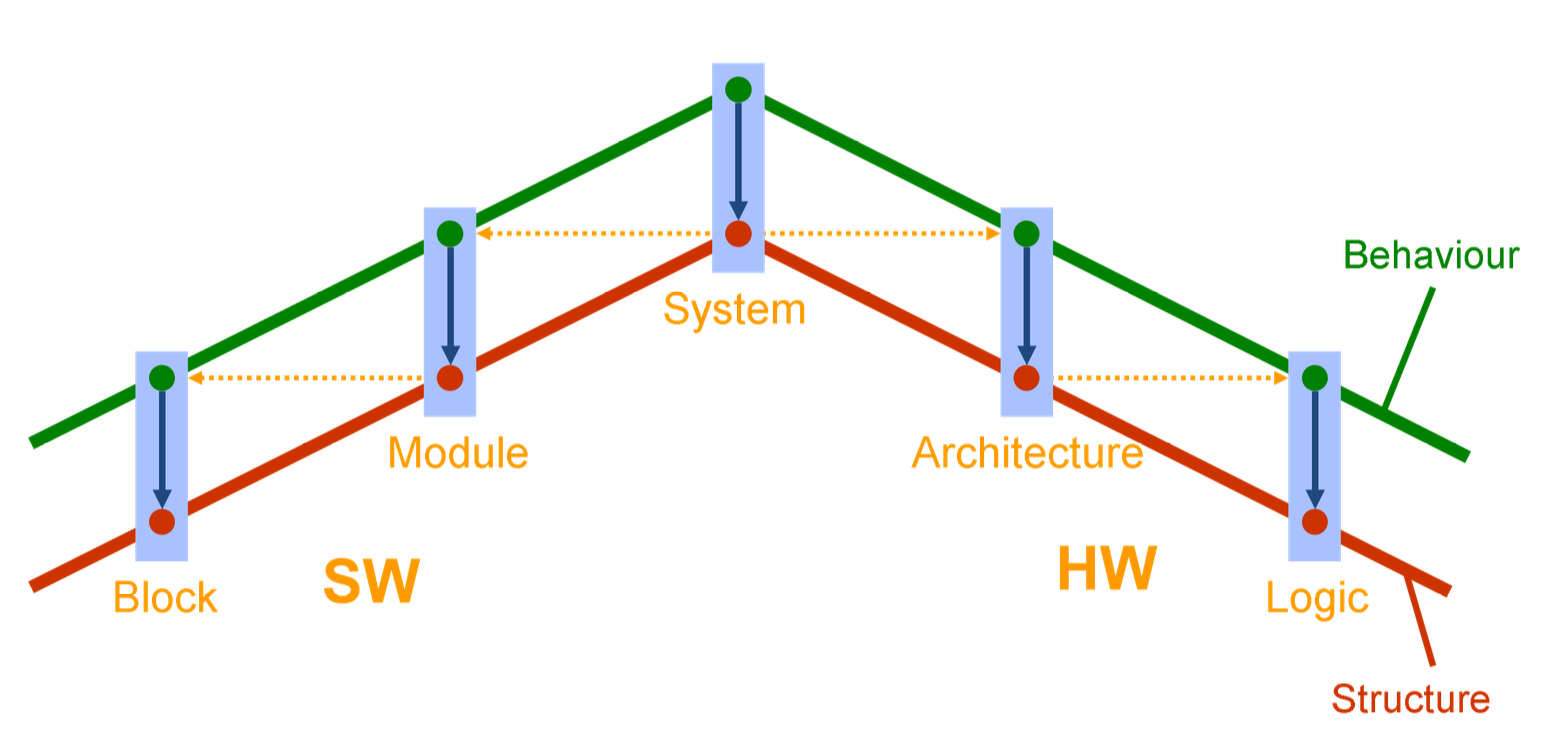
\includegraphics[width=0.5\textwidth]{images/Double_roof.png}
		\caption{Double Roof}
		\label{fig:double_roof}
	\end{center}
\end{figure}
\subsection{Compiler - Basics}
\begin{figure}[h]
	\begin{center}
	\begin{subfigure}[b]{0.4\textwidth}
		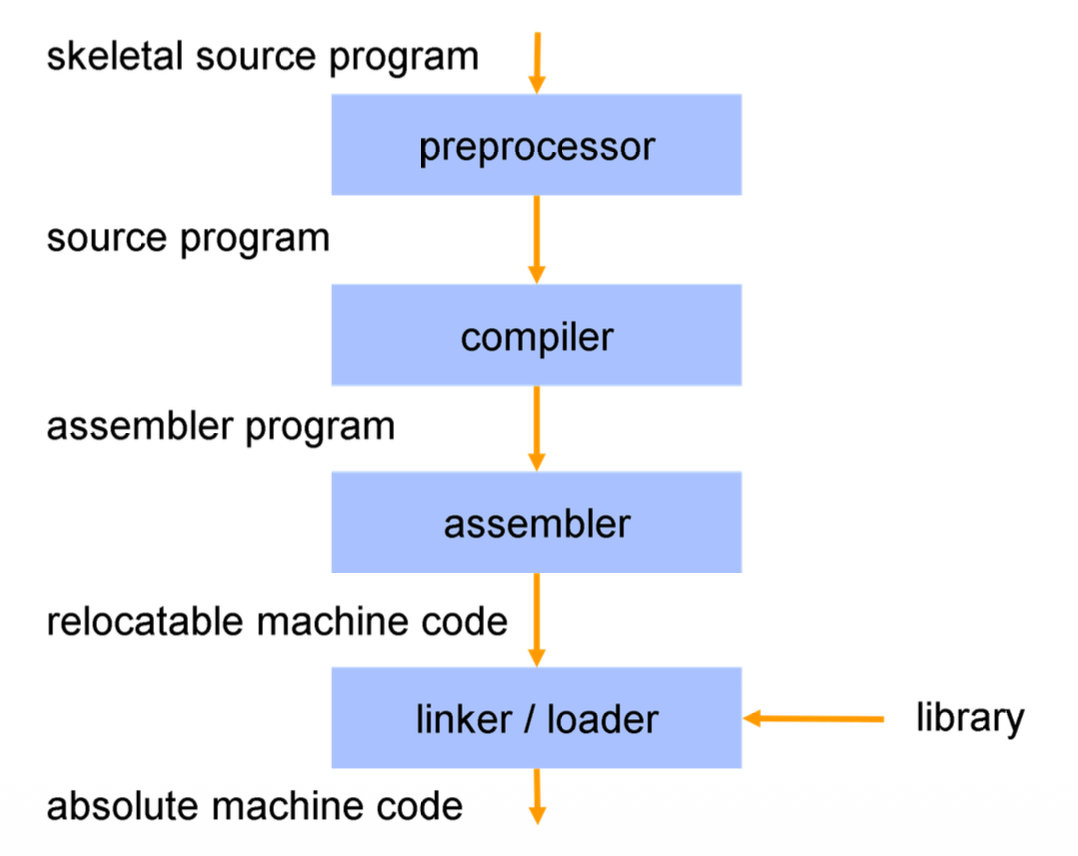
\includegraphics[width=\textwidth]{images/Compilation_process.png}
		\caption{Compilation Process}
		\label{fig:comp_process}
	\end{subfigure}
	\hfill
	\begin{subfigure}[b]{0.5\textwidth}
		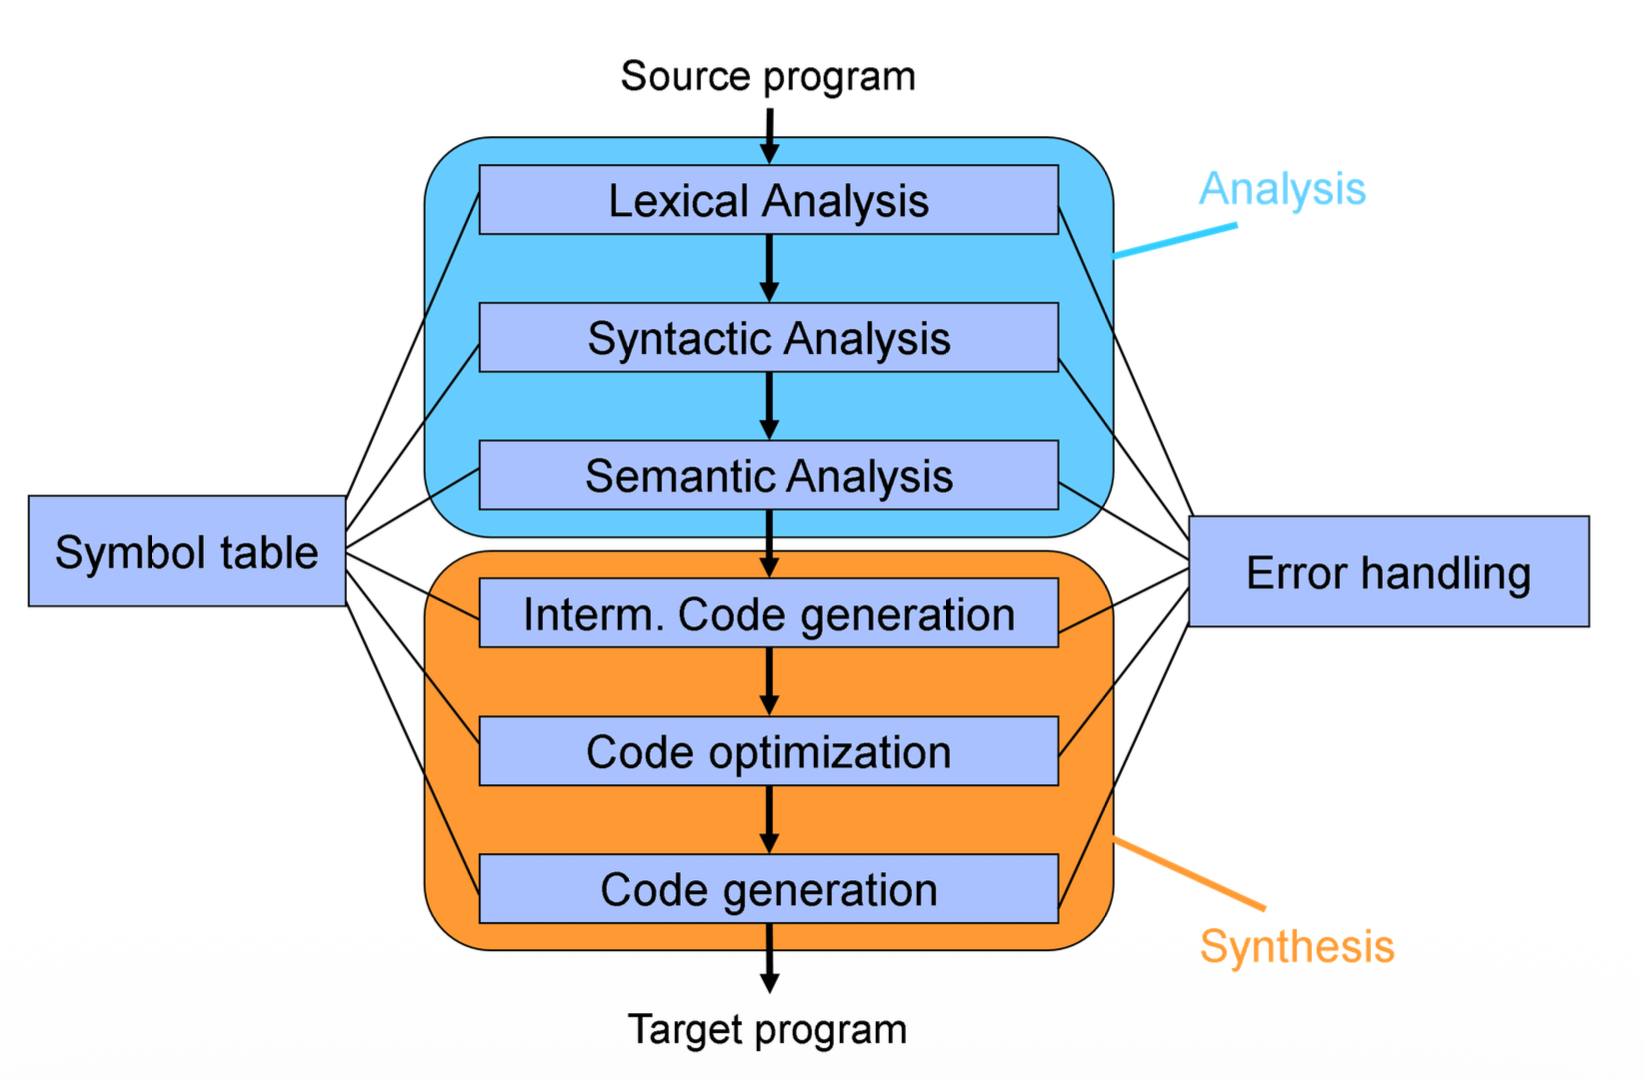
\includegraphics[width=\textwidth]{images/Compilor_phases.png}
		\caption{Compilation Process}
		\label{fig:comp_process}
	\end{subfigure}
	\caption{Compiler}
\end{center}
\end{figure}

\subsubsection{Analysis}
\begin{itemize}
	\item Lexical Analysis
\begin{itemize}
	\item scan source program and decompose it into symbols 
	\item regular expression: recognition through finite automata 
\end{itemize}
\item syntactic analysis
\begin{itemize}
	\item parse sequences of symbols and determine clauses
	\item clauses are described by a context free grammar
\begin{itemize}
	\item Z $\rightarrow$ Identifier $:=$ A
	\item A $\rightarrow$ A + A $|$ A * A $|$ Identifier $|$ Number
\end{itemize}
\end{itemize}
\item semantic analysis
\begin{itemize}
	\item assure that the pieces fit together semantically
	\item Example: type conversion
\end{itemize}
\end{itemize}

\begin{figure}[h]
	\begin{center}
		\begin{subfigure}[b]{0.5\textwidth}
			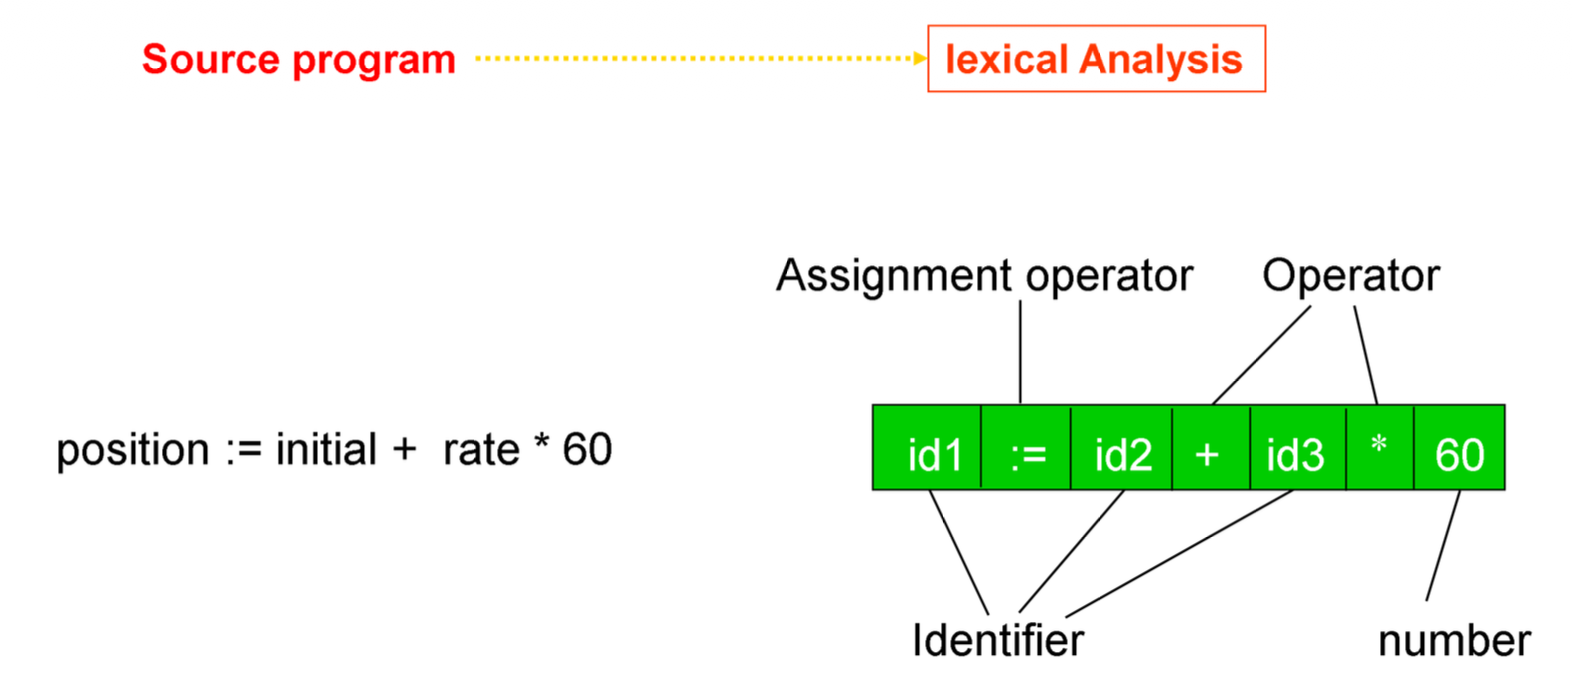
\includegraphics[width=\textwidth]{images/Analysis_1.png}
		\end{subfigure}
		\hfill
		\begin{subfigure}[b]{0.4\textwidth}
			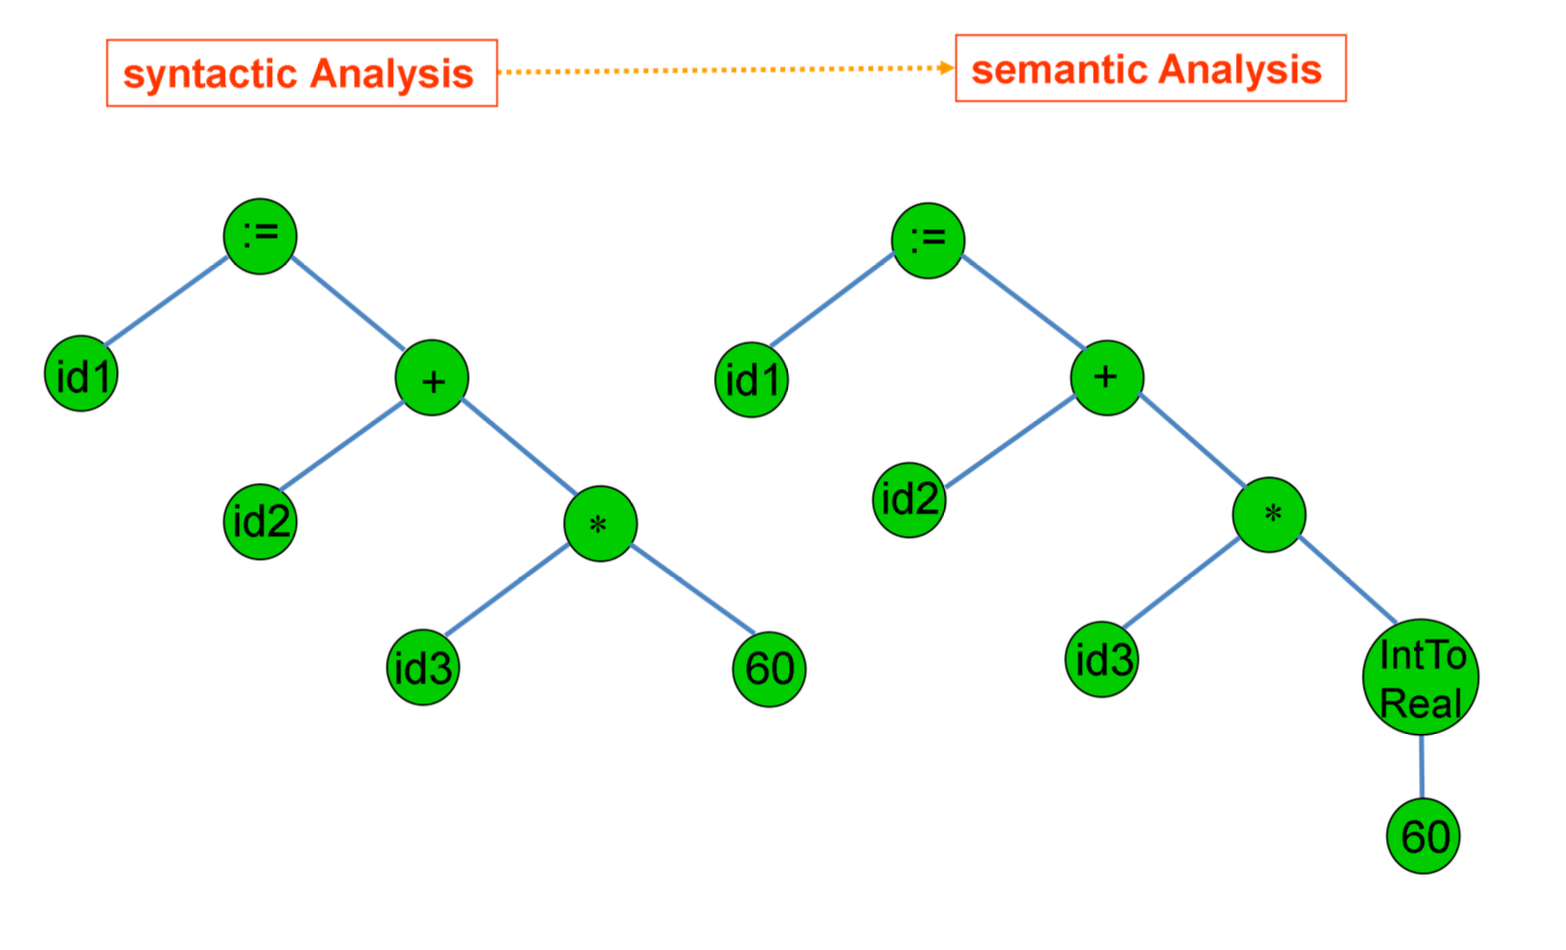
\includegraphics[width=\textwidth]{images/Analysis_2.png}			
		\end{subfigure}
		\caption{Analysis Example}
		\label{fig:analysis}
	\end{center}
\end{figure}

\subsubsection{Synthesis}
\begin{itemize}
	\item Generation of intermediate code
\begin{itemize}
	\item machine independent $\rightarrow$ retargeting easier
	\item easy to generate
	\item easy to be translated 
\end{itemize}
\item Optimization
\begin{itemize}
	\item General-purpose processors: fast code, fast translation
	\item Special processors: fast code, compact code, small memory image
	\item of intermediate code or of target code
\end{itemize}
\item Code generation
\end{itemize}

\begin{figure}[h]
	\begin{center}
		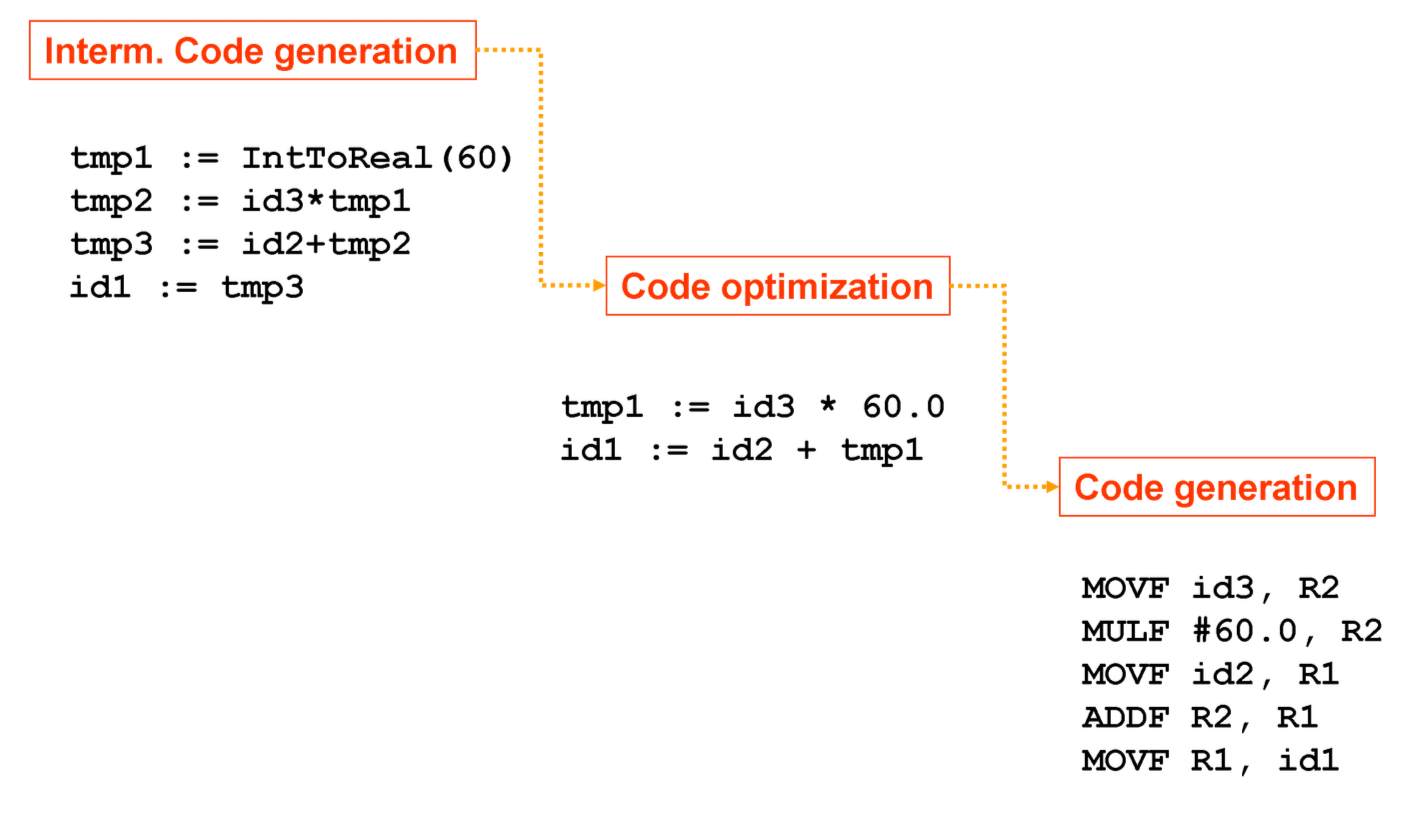
\includegraphics[width=0.5\textwidth]{images/Synthesis.png}
		\caption{Synthesis Example}
		\label{fig:synthesis}
	\end{center}
\end{figure}

\subsubsection{Syntax Tree abd DAG}
\begin{figure}[h]
	\begin{center}
		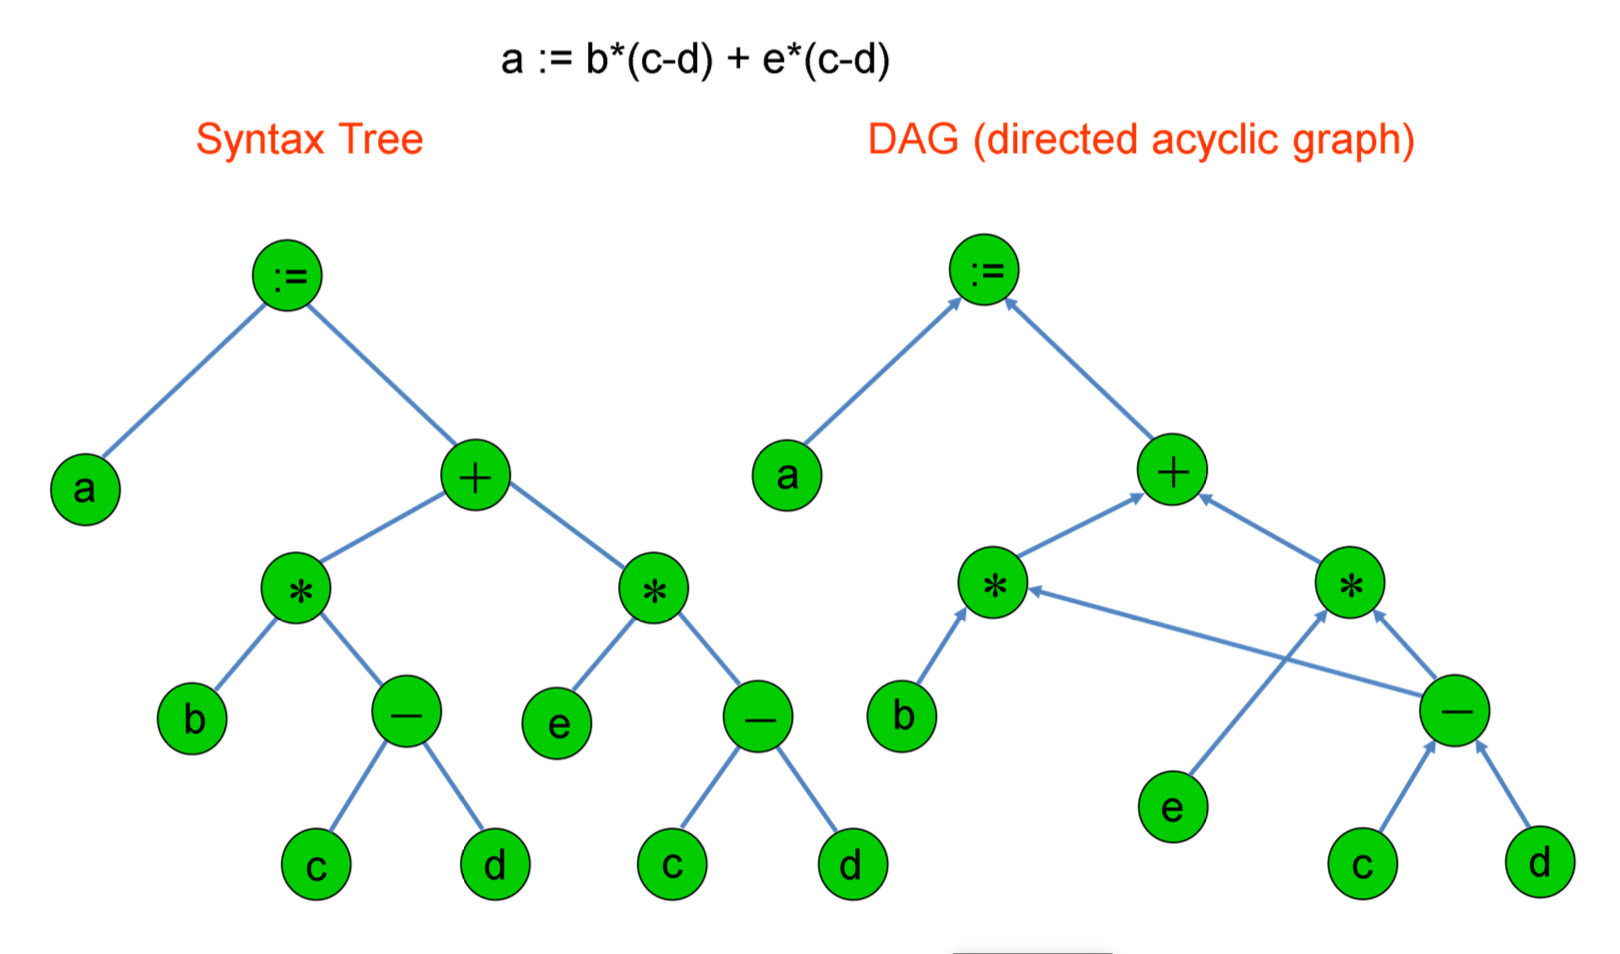
\includegraphics[width=0.5\textwidth]{images/Syn_and_DAG.png}
		\caption{Syntax Tree and DAG}
		\label{fig:syn_and_DAG}
	\end{center}
\end{figure}


\subsubsection{3-Address Code}
\begin{itemize}
	\item Instructions
\begin{itemize}
	\item maximum 3 addresses (2 operands, 1 result)
	\item maximum 2 operants
\end{itemize}
\item Assignments
\begin{itemize}
	\item \begin{verbatim} x := y op z\end{verbatim}
	\item \begin{verbatim} x := op y\end{verbatim}
	\item \begin{verbatim} x := y\end{verbatim}
	\item \begin{verbatim} x := y[i]\end{verbatim}
	\item \begin{verbatim} x[i] := y\end{verbatim}
	\item \begin{verbatim} x := &y\end{verbatim}
	\item \begin{verbatim} y := *x\end{verbatim}
	\item \begin{verbatim} *x := y\end{verbatim}
\end{itemize}
\item Control flow
\begin{itemize}
	\item \begin{verbatim} goto L\end{verbatim} 
	\item \begin{verbatim} if x relop y goto L	\end{verbatim}
\end{itemize}
\item Sub programs
\begin{itemize}
	\item \begin{verbatim} param x\end{verbatim}
	\item \begin{verbatim} call p,n\end{verbatim}
	\item \begin{verbatim} return y\end{verbatim}
\end{itemize}
\item Advantages
\begin{itemize}
	\item resolution of lengthy expressions and nested loops
	\item temporary names allow for easy reordering
	\item represents already a valid schedule
\end{itemize}
\item Definition
\begin{itemize}
	\item \begin{verbatim} x := y op z\end{verbatim}
	\item defines x and uses y and z
\end{itemize}
\end{itemize}

\begin{figure}[h]
	\begin{center}
		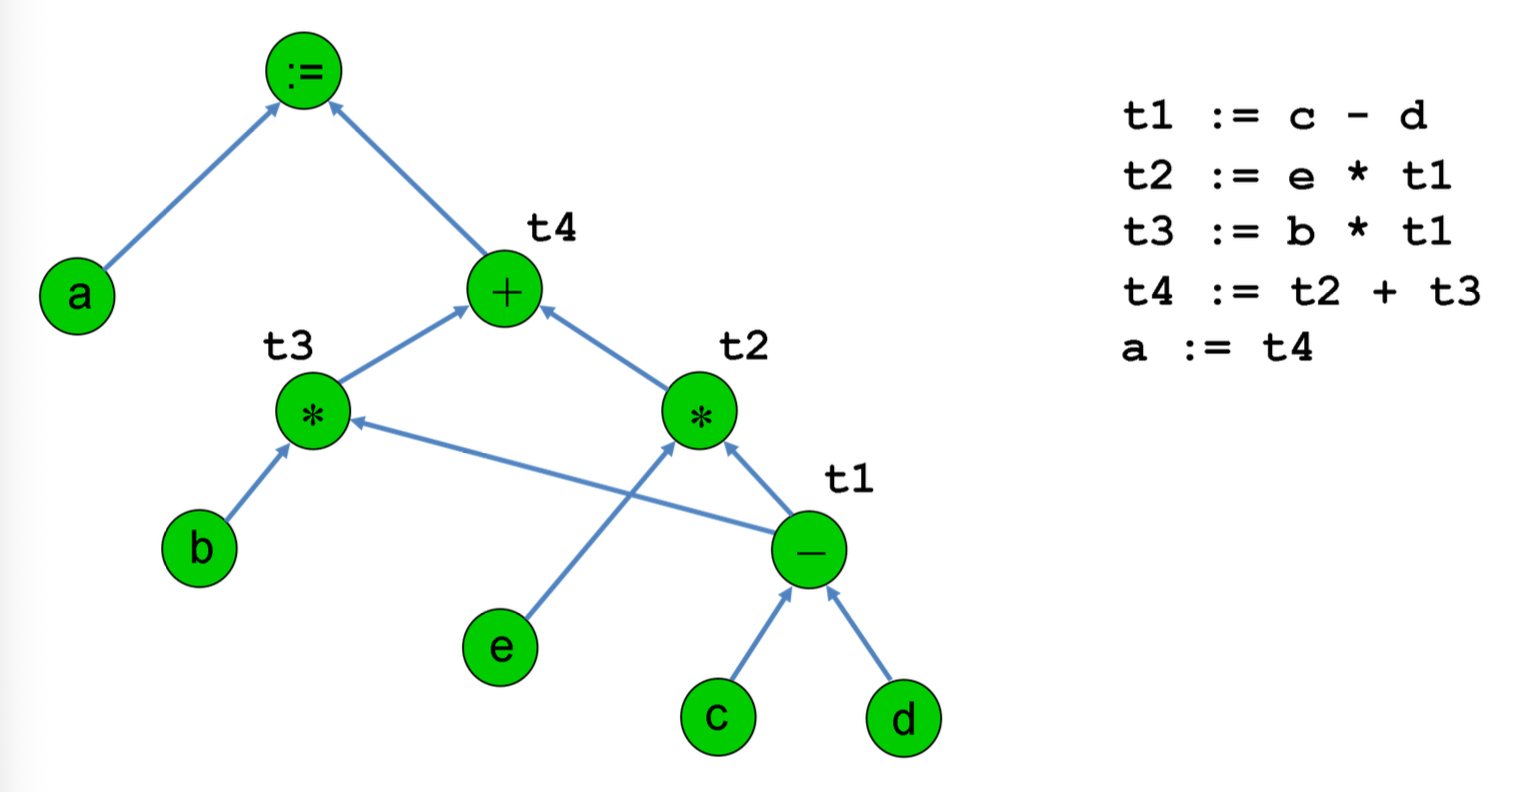
\includegraphics[width=0.5\textwidth]{images/3-address.png}
		\caption{Generation of 3-address-code from DAG}
		\label{fig:3-address}
	\end{center}
\end{figure}

\subsubsection{Basic Block}
Definition: A basic block is a sequence of consecutive instructions in which the control flow enters at the beginning and leaves at the end without branching except at the end.

Sequence of 3-address instructions $\rightarrow$ set of basic block:
\begin{enumerate}
  \item Determine block start points:
\begin{itemize}
	\item the first instruction
	\item targets of branch and jump instructions
	\item instructions directly following a branch or jump instruction
\end{itemize}
\item Determination of basic blocks
\begin{itemize}
	\item each basic block includes its block start point
	\item includes all instructions (but excluding) the next block start point or until the program ends
\end{itemize}

\end{enumerate}

\subsubsection{CFG and DAG for basic blocks}
\begin{figure}[h]
	\begin{center}
	\begin{subfigure}[b]{0.45\textwidth}
		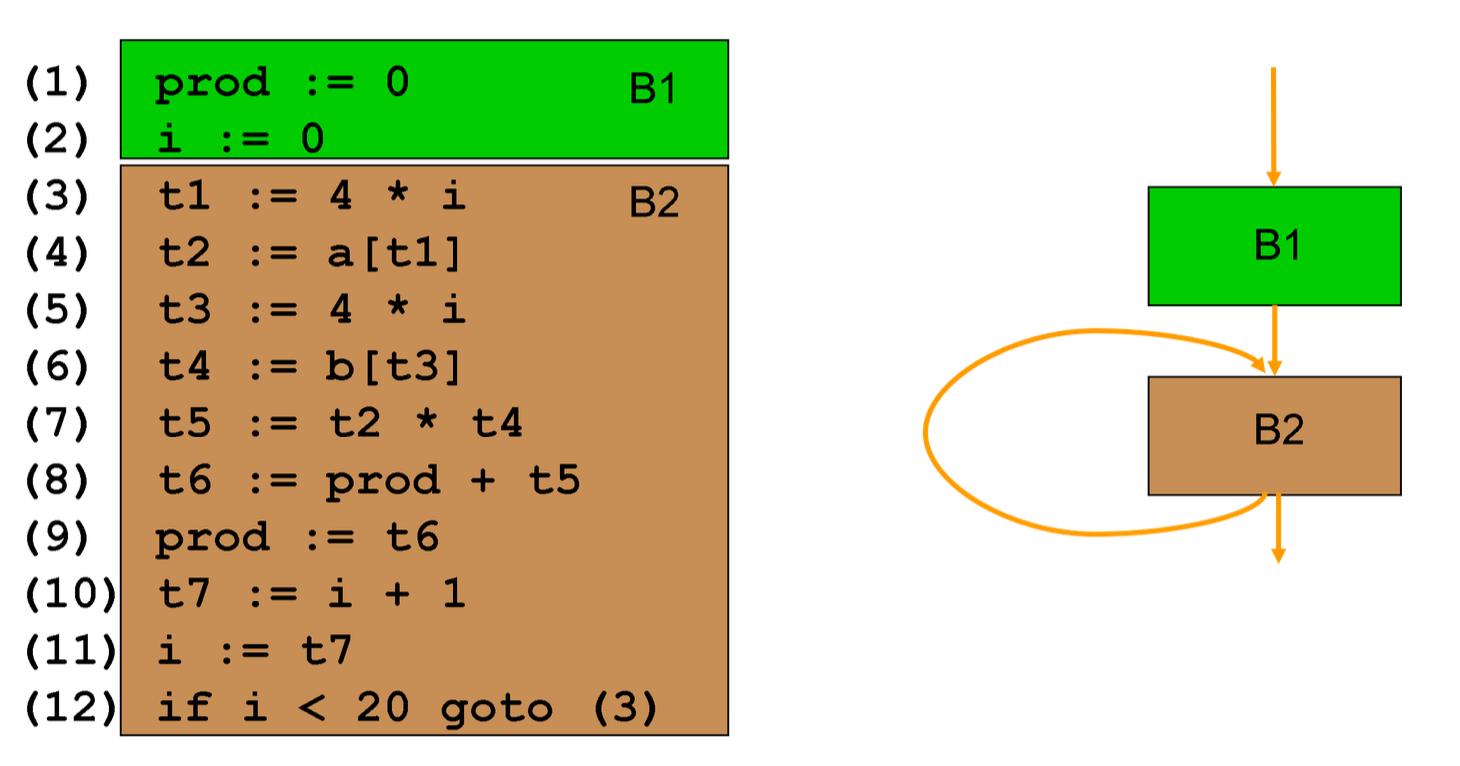
\includegraphics[width=\textwidth]{images/Degen_CFG.png}
		\caption{Degenerated Control Flow Graph}
		\label{fig:degen_CFG}
	\end{subfigure}
	\hfill
	\begin{subfigure}[b]{0.45\textwidth}
		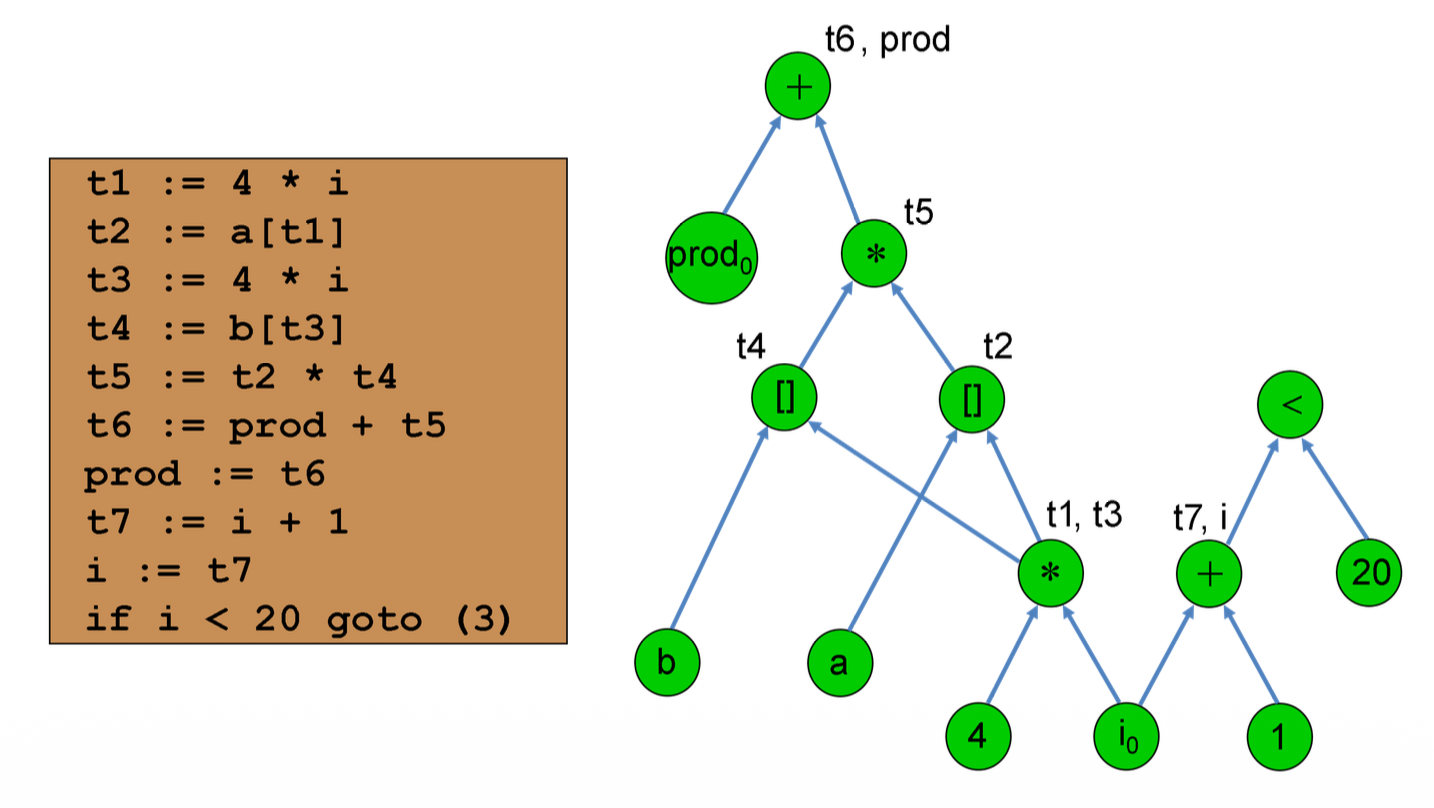
\includegraphics[width=\textwidth]{images/DAG_bb.png}
		\caption{Directed acyclic graph}
		\label{fig:DAG_basic_block}
	\end{subfigure}
	\caption{CFG and DAG for basic blocks}
	\end{center}
\end{figure}

\subsection{Code generation}
\begin{itemize}
	\item Requirements
\begin{itemize}
	\item correct code
	\item efficient code
	\item efficient code generation
\end{itemize}
\item Code generation = Software synthesis
\begin{itemize}
	\item Allocation: often given
	\item Binding:
\begin{itemize}
	\item Register allocation, register binding
	\item Code (instruction) selection
\end{itemize}
\item Scheduling
\begin{itemize}
	\item Instruction sequencing
\end{itemize} 
\end{itemize}
\item Goal: efficient register usage
\begin{itemize}
	\item instructions on register operands typically shorter and faster as instructions with memory operands
\end{itemize}
\item Register allocation, register binding
\begin{itemize}
	\item determine at each point of the program the set of variables hat shall be stored in a register
	\item bind each variable to a physical register
	\item optimal register binding in a NP-complete problem
	\item additional constrains given by special registers of the CPU architecture, compiler and operating system
\end{itemize}
\end{itemize}

\subsubsection{Code (Instruction) Selection}
\begin{itemize}
	\item Code pattern for implementing a 3-address instruction [\cref{fig:3-addres_to_assembler}]
	\item Problems
\begin{itemize}
	\item often inefficient code $\rightarrow$ Code optimization
	\item There may be many alternative instructions
	\item some instructions are only executable on certain registers
	\item exploitation of special processor properties   
\end{itemize}
\end{itemize}

\begin{figure}[h]
	\begin{center}
		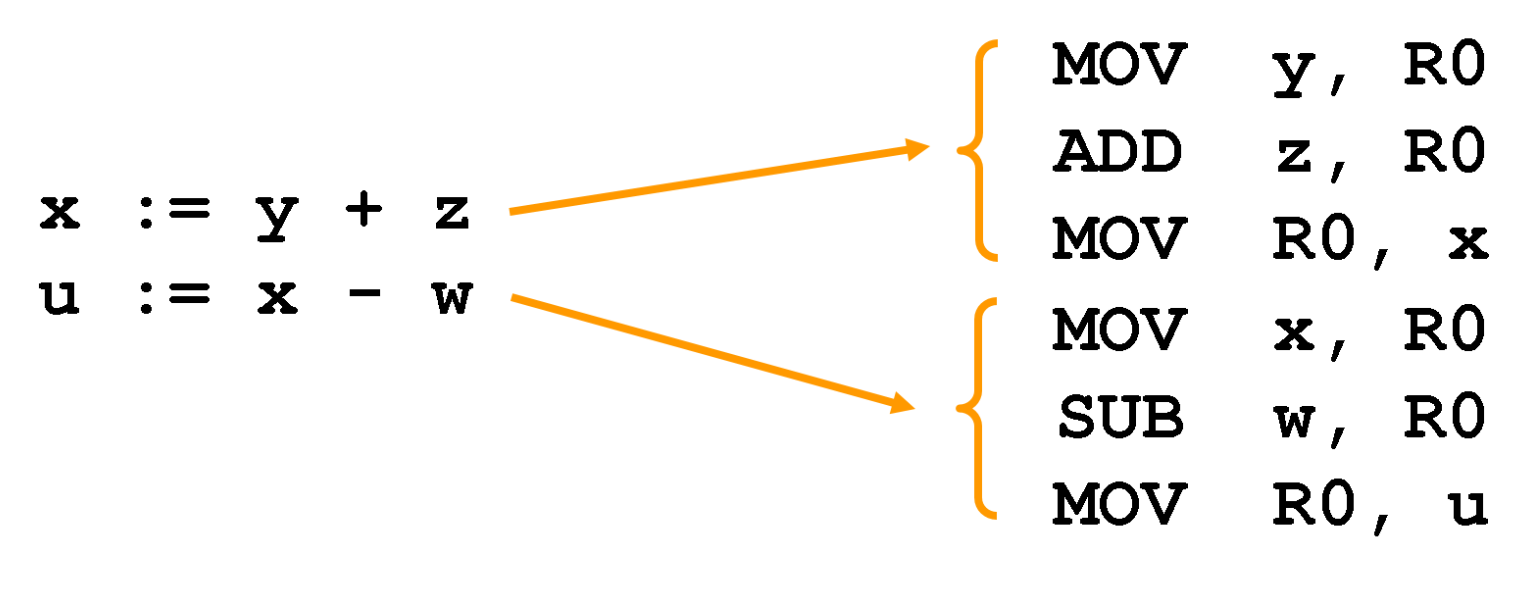
\includegraphics[width=0.5\textwidth]{images/Code_selection.png}
		\caption{3-address to assembler}
		\label{fig:3-addres_to_assembler}
	\end{center}
\end{figure}

\subsubsection{Scheduling}
Goal: efficient instruction execution sequences, as short as possible, using few registers

\begin{figure}[h]
	\begin{center}
		\begin{subfigure}[b]{0.55\textwidth}
			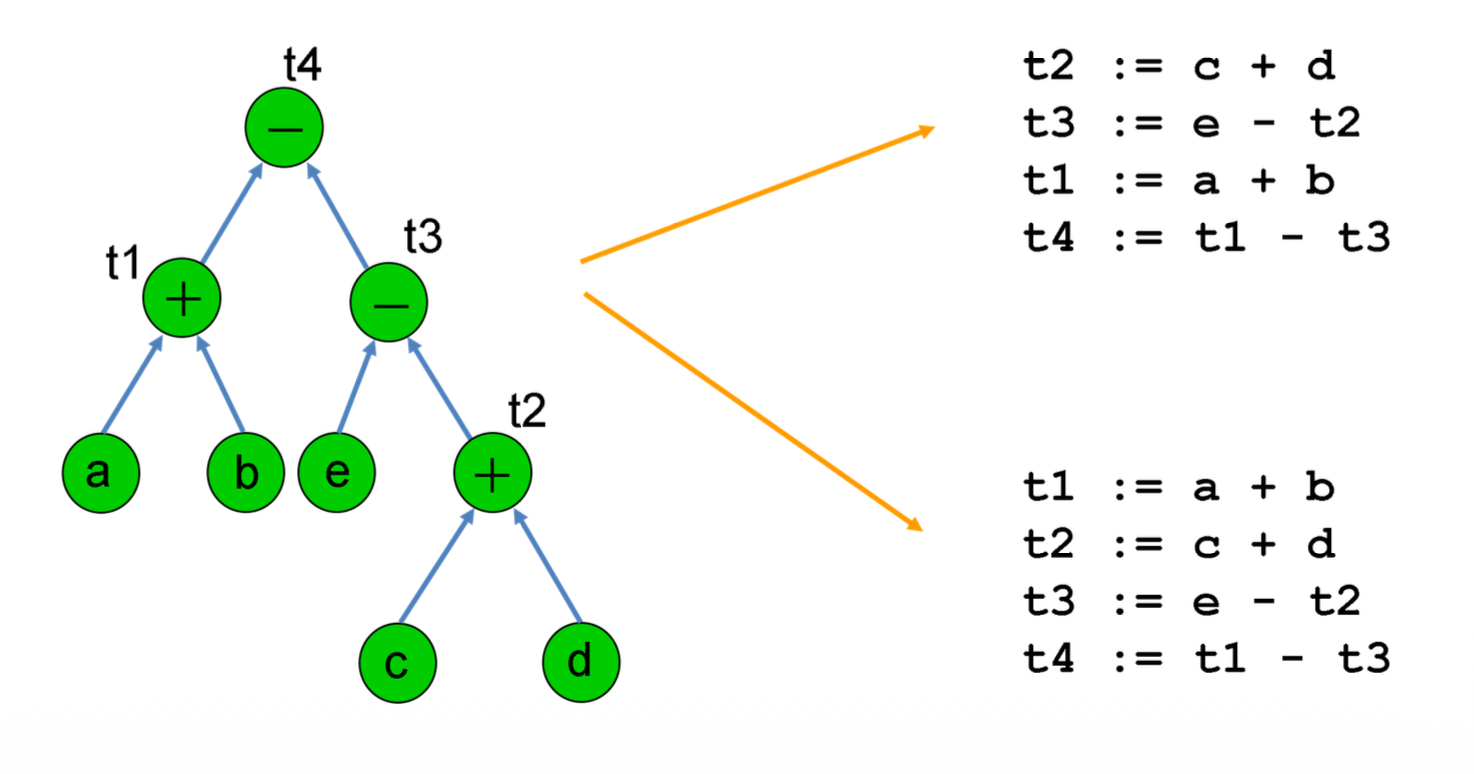
\includegraphics[width=\textwidth]{images/Scheduling_1.png}
		\end{subfigure}
		\hfill
		\begin{subfigure}[b]{0.35\textwidth}
			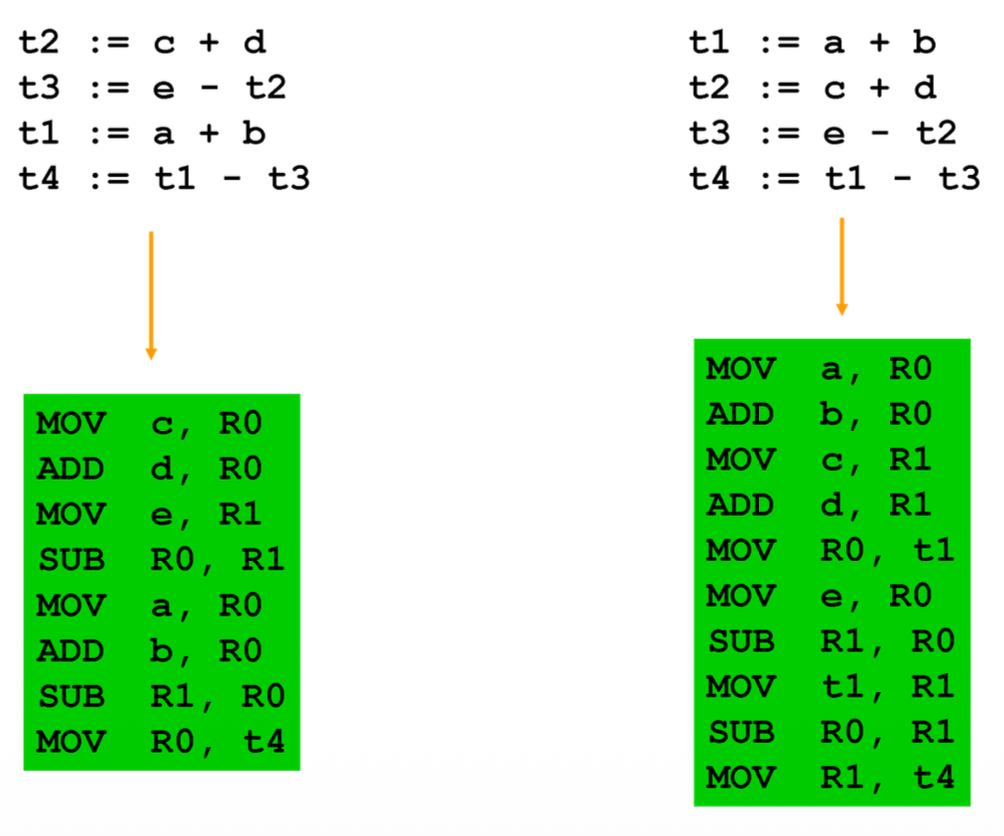
\includegraphics[width=\textwidth]{images/Scheduling_2.png}
		\end{subfigure}
		\caption{Scheduling differences}
		\label{fig:scheduling}
	\end{center}
\end{figure}



 


